%!TEX encoding = UTF-8 Unicode
%!TEX root = ../lect-w11.tex

%%%

% \ifkompendium\else
% \begin{SlideExtra}{Kom på föreläsning om systemutveckling!}
% \begin{itemize}
%   \item \Alert{12/12 kl 13-15 i E:C} ger Björn Regnell en föreläsning i C:arnas kurs om digitalisering EITA65: 
% \begin{itemize}
%   \item \Emph{Kravhantering} för mjukvara: hur bestämma vad koda?
%   \item Hur bäst dra nytta av \Emph{öppen källkod}?
% \end{itemize}
%   \item Alla \Alert{D-are} är också \Emph{hjärtligt välkomna!!!}
% \end{itemize}
  
% \end{SlideExtra}
% \fi 

\Subsection{Om projektuppgiften}

\begin{Slide}{Om din avslutande projektuppgift}\SlideFontSmall
\Emph{Läs noga kompendium Del 1, kapitel -1 avsnitt ''Projektuppgift''!} \\
Några viktiga punkter:
\begin{itemize}
\item Mål: skapa ett stort program med många samverkande klasser/moduler.
\item Projektet går över \Alert{två veckor}. Schemalagda labbar i december är \Alert{obligatoriska} för de som har kvar obligatoriska moment.

\item I kompendium Del 2, kapitel 13, finns flera förslag att välja bland.

\item Inför redovisningen ska du skapa automatiskt genererad dokumentation utifrån relevanta dokumentationskommentarer för minst hälften av dina publika metoder, enligt instruktioner i Appendix E.

\item Redovisning sker i datorsal på schemalagd tid:
\begin{itemize}\SlideFontTiny
  \item Förklara hur din kod fungerar.
  \item Beskriv framväxten av ditt program.
  \item Gå igenom den genererade dokumentationen av din kod.
\end{itemize}
\end{itemize}

\end{Slide}

\begin{Slide}{Projektuppgifter}\SlideFontTiny
Om du inte vet vilken du ska välja så välj gärna \code{bank} som tränar grunderna.
\begin{itemize}\SlideFontTiny
\item \code{bank}
\begin{itemize}\SlideFontTiny
\item känd domän: skapa bank med transaktionshistorik 
\item oföränderlig data tillsammans med tillståndsförändring
\end{itemize}

% \item \code{tabular}
% \begin{itemize}\SlideFontTiny
% \item behandling av data i tabellform 
% \item matris, oföränderlig data
% \end{itemize}

\item \code{music}
\begin{itemize}\SlideFontTiny
\item skapa ett enkelt kompositionsverktyg som spelar musik
\item sätta sig in i en domänmodell
\end{itemize}

\item \code{photo} 
\begin{itemize}\SlideFontTiny
\item en enkel variant av photoshop 
\item inblick i grundläggande matrismatematik
\end{itemize}


\item egendefinierat projekt 
\begin{itemize}\SlideFontTiny
\item Lagom svårt: ej för enkel uppgift, men ta dig inte vatten över huvudet!
\item Diskutera med en handledare och dokumentera egna uppgiften och dess omfattning och relation till lärandemålen i kursen så att andra handledare och kursansvarig kan förstå varför projektet passar i kursen.
\item Du måste få OK från en handledare innan du startar egendefinierat projekt.
\end{itemize}


\end{itemize}

\end{Slide}

\begin{Slide}{Skapa dokumentation}
Med \code{scala doc} . kan du ta dokumentationskommentarerna i källkoden och skapa en webbsajt med dokumentation.

\vspace{2em}
\begin{tikzpicture}[node distance=1.5cm,scale=0.8, every node/.style={transform shape}]

\node (input) [startstop] {\texttt{.}};

\node(inptext) [right of=input, text width=4cm, scale=1.2,xshift=4.5cm]{Aktuell katalog med \texttt{.scala}-filer};

\node (scaladoc) [process, below of=input]
{\texttt{scala doc .}};

\node (output) [startstop, below of=scaladoc] {\texttt{./scala-doc}};

\node(outtext) [right of=output, text width=4cm, scale=1.2,xshift=4.5cm]{\texttt{index.html} och en massa andra filer som ger en hel webbsajt!};


\draw [arrow] (input) -- (scaladoc);
\draw [arrow] (scaladoc) -- (output);
\end{tikzpicture}

\vspace{1em} Öppna \texttt{scala-doc/index.html} i en webbläsare.
\end{Slide}
  
  

\begin{Slide}{Dokumentationskommentarer}\footnotesize
För att kod ska bli begriplig för människor är det bra att dokumentera vad den gör. Det finns \Emph{tre olika sorters kommentarer}:
\begin{lstlisting}
// Enradskommentarer börjar med dubbla snedstreck
//       men de gäller bara till radslut

/* Flerradskommentarer börjar med
   snedstreck-asterisk
   och slutar med asterisk-snedstreck.  */

/** Dokumentationskommentarer placeras före
 *   t.ex. en funktion och berättar vad den gör
 *   och vad eventuella parametrar används till.
 *   Börjar med snedstreck-asterisk-asterisk.
 *   Varje ny kommentarsrad börjar med asterisk.
 *   Avslutas med asterisk-stjärna.
 */
\end{lstlisting}
Kommentarer påverkar inte hur maskinen exekverar koden, men hjälper människor att använda koden och verktyg att visa hjälp. Se Appendix E.
\end{Slide}

\ifkompendium\else


\Subsection{Obligatorisk munta, valfri tenta}


\begin{SlideExtra}{Avslutning och uppsamling}

\begin{itemize}\SlideFontSmall

\item Gör en \Alert{detaljerad} plan dag-för-dag för din kursavslutning.

\item Schematider i \Alert{sista läsveckan} är till för \Emph{muntligt prov, projektredovisning, redovisning av restlabbar}.

\item Det är ok att redovisa projekt och göra munta tidigare i mån av plats. \\Men PLUGGA NOGA inför muntan!!! (Se nästa slajd.)

\item Alla obl. labbar klara innan du muntar. OK munta under projektarbetet.

\item \Emph{Godkänd} grundkurs är \Alert{krav} för att få påbörja efterföljande \code{pfk}.

\item \Emph{Kolla din status i SAM}. Se i Canvas hur du loggar in i SAM.
\end{itemize}

\end{SlideExtra}

\begin{SlideExtra}{Obligatoriskt muntligt prov}
\begin{itemize}\SlideFontSmall
  \item Syftet med det muntliga provet är att säkerställa att alla som påbörjar efterföljande kurs har tillräckliga \Emph{grundkunskaper}, med fokus på \Emph{konceptuell förståelse} och förmåga att \Alert{självständigt} \Emph{skapa kod}.
  \item Det muntliga provet tar mellan 10 och 30 min beroende på hur många frågor handledare behöver ställa för att kunna kan avgöra om du har tillräcklig förståelse. Vid osäkerheter tar kursansvarig över.
  \item Enda tillåtna hjälpmedel: snabbref, och på anmodan av handledare även REPL. Medtag papper och penna!
  \item \Alert{Alla obl. labbar måste vara godkända} innan du får göra  provet.
  \item Det är ok att göra det muntliga provet även innan projektet är klart.
  \item Om du är godkänd på alla obligatoriska moment får du minst 3:a i kursen och du har då klarat förkunskapskraven för efterföljande kurser.
  \item Du ber handledare att få göra muntligt prov på samma sätt som du tidigare bett om att få redovisa labbar. Munta sker på plats i datorsal.
  \item Träna på provet här: \url{https://fileadmin.cs.lth.se/pgk/muntabot}
\end{itemize}  
\end{SlideExtra}

\begin{SlideExtra}{Gör den valfria tentan!}
\begin{itemize}\SlideFontSmall
  \item \Emph{Alla} som kan \& vill uppmuntras göra den valfria tentan!
  \item \Alert{Alla} obligatoriska moment måste vara klara innan du får tentera.
  \item Den valfria tentan ger högre betyg om du klarar gränserna för 4:a el. 5:a.
  \item Tentan liknar de extentor som finns på kurshemsidan.
  \item Tentan är på plats och skrivs med papper och penna. 
  \item Enda hjälpmedel: snabbreferensen.
  \item Snabbreferens beställs i Canvas och hämtas hos \url{birger.swahn@cs.lth.se}
  \item Tentan ges en gång om året i januari. Det är tillåtet att ''plussa'' ett senare år om du inte är nöjd med ditt betyg.
  \item \Alert{OBS! Obligatorisk anmälan} i LTH:s ordinarie tentasystem. \\ %Anmälningssystemet är öppet sedan i går och stänger den 14/12.
  \url{https://www.student.lth.se/mina-studier/tentamen/} 
\end{itemize}
\end{SlideExtra}


\begin{Slide}{Tips: Före tentan}\SlideFontSmall
\begin{enumerate}
\item Repetera övningar och labbar i kompendiet.
\item Läs igenom föreläsningsanteckningar.
\item Studera \Emph{snabbref} \Alert{mycket noga} så att du vet vad som är givet och var det står, så att du kan hitta det du behöver snabbt.
\item Skapa och \Emph{memorera} en personlig \Emph{checklista} med programmeringsfel du brukar göra, som även inkluderar småfel, så som glömda parenteser och semikolon, och annat som en kompilator/IDE normalt hittar.
\item Tänk igenom hur du ska disponera dina 5 timmar på tentan.
\item Gör minst en extenta som om det vore \Alert{skarpt läge}:
\begin{enumerate}\SlideFontTiny
\item Avsätt 5 ostörda timmar (stäng av telefon, dator etc).
\item Inga hjälpmedel. Bara snabbref.
\item Förbered dryck och tilltugg.
\end{enumerate}
\end{enumerate}
\end{Slide}

\begin{Slide}{Tips: På tentan} \SlideFontTiny
\begin{enumerate}
\item Läs igenom \Alert{hela} tentan först. \\ \Emph{Varför?} Förstå helheten. Delarna hänger ihop.
\item Notera och begrunda specifika begrepp och definitioner. \\ \Emph{Varför?} Begreppen är avgörande för förståelsen av uppgiften.
\item Notera förenklingar, antaganden och specialfall. \\ \Emph{Varför?} Uppgiften blir mkt enklare om du inte behöver hantera dessa.
\item \Alert{Fråga} tentamensansvarig om du inte förstår uppgiften -- speciellt om det finns misstänkta felaktigheter eller förmodat oavsiktliga oklarheter. \\ \Emph{Varför?} Det är inte lätt att konstruera en ''perfekt'' tenta. \\ Du får fråga vad du vill, men det är inte säkert du får svar...
\item Läs specifikationskommentarerna och metodsignaturerna i alla givna klass-specifikationer \Alert{mycket noga}. \\ \Emph{Varför?} Det är ett vanligt misstag att förbise de ledtrådar som ges där.
\item Återskapa din memorerade personliga checklista för vanliga fel som du brukar göra och avsätt tid till att gå igenom den på tentan. Varje fix plockar poäng!
\item Lämna in ett försök även om du vet att lösningen inte är fullständig. Det gäller att plocka så många poäng det går. En ofullständig lösning kan ändå ge poäng.

\item Om du har svårigheter kan det bli kamp mot klockan. Försök hålla huvudet kallt och prioritera utifrån var du kan plocka flest poäng. Ge inte upp! Ta en kort äta-dricka-paus för att få mer energi!

\end{enumerate}
\end{Slide}

\begin{Slide}{Tentans struktur}
\begin{itemize}\SlideFontSmall
\item Del A 20\%:\\\Emph{Evaluera uttryck} där du ska \Alert{ange typ och värde}
\begin{itemize}\SlideFontTiny
\item Testar förståelse av variabler, uttryck, samlingar, algoritmer, arv, etc.
\item Det är bra/nödvändigt att anteckna delsteg och variablers värden, då det är mycket svårt att tänka ut svaren direkt i huvudet.
\item Du måste träna mycket på denna del i förväg för att ha god chans att plocka många poäng, se extentor.
%\item Ev. ''rättningströskel'': \textit{Om du på del A erhåller färre poäng än vad som krävs för att nå upp till en bestämd ''rättningströskel'', kan din tentamen komma att underkännas utan att del B bedöms.}
\end{itemize}


\item Del B 80\%:\\\Emph{Skriva kod} som uppfyller \Alert{krav och design}
\begin{itemize}\SlideFontTiny
\item Testar att du själv kan skapa kod med delar som samverkar
\item Testar förmåga att gå från indata-utdata till algoritm \\
 givet: ledtrådar, design, ev. skiss på lösning, ev. pseudokod etc.
\end{itemize}
\item Blanka inlämningar ger 0 poäng; det är alltid bättre att försöka än att lämna in blankt. Lämna inte in kladdpapper eller dubbla lösningar.
\end{itemize}
\end{Slide}

% \Subsection{Grumligt-lådan \& Nyfiken-på-lådan}
% \begin{Slide}{Grumligt-lådan och Nyfiken-på-lådan}
% \begin{itemize}
% \item Skriv lapp i \Alert{GRUMLIGT}-lådan om du har något \Alert{grundläggande begrepp} i kursen som du fortfarande tycker är \Alert{svårt att begripa}.
%
% \item[]
%
% \item Skriv lapp i \Emph{NYFIKEN-PÅ}-lådan om du vill veta mer om något ämne inom programmering och som går \Emph{bortom grunderna}.
% \end{itemize}
% \end{Slide}

\Subsection{CEQ}


\begin{Slide}{CEQ -- Course Experience Questionnaire}\SlideFontSmall
\begin{itemize}
\item Görs på hela LTH på samma sätt. Alla får länkar via mejl.
\item Snälla fyll i CEQ! Jag är \Alert{mycket tacksam} för all konstruktiv feedback! \\ Hög svarsfrekvens är viktigt för att kunna dra slutsatser om variationen i svaren och signifikansen i sammanställningen.
\item Del 1: Generella påståenden, alla med 5-gradig skala: \\ tar helt avstånd ... instämmer helt
\item Del 2: \Emph{Fritextfrågor}: \\
''Vad  tycker  du  var  det  bästa  med  den här  kursen?'' \\
''Vad  tycker  du  främst  behöver  förbättras?''
\item Mer om CEQ här: \url{https://www.ceq.lth.se/}
%\item \Emph{Fördel} med CEQ: Samma alla kurser alla år medger jämförelse över tid.
%\item \Alert{Begränsning}: Saknar frågor kopplat till specifika kursmoment.
\end{itemize}
\end{Slide}

% \begin{Slide}{Kursspecifik utvärdering om specifika kursmoment}\SlideFontSmall
% \begin{itemize}
% \item Jag vill gärna att \Alert{alla} gör den LTH-gemensamma, anonyma kursutvärderingsenkäten \href{https://www.ceq.lth.se/}{CEQ}. Dina fritext-kommentarer om vad som är det bästa med kursen och vad som främst behöver förbättra emottages mycket tacksamt i CEQ-utvärderingen!
% \item Jag kommer att komplettera CEQ med en \Emph{kursspecifik utvärdering} av specifika kursmoment i denna kurs och jag är därför \Alert{mycket tacksam} om alla fyller enkäten när länk kommer via anslag i Canvas.
% \item Jag behandlar dina svar \Alert{konfidentiellt}, men sparar din email så att jag kan återkomma om jag mot förmodan undrar något mer.
% \item Din input är \Emph{mycket värdefull} vid framtida kursutveckling!
% \end{itemize}
% \end{Slide}

\Subsection{Avslutning}

\begin{Slide}{När du om några år tänker tillbaka på pgk...}
...hoppas jag du uppskattar den allmänbildning du fick om:
\begin{itemize}
  \item sekvens -- alternativ -- repetition -- abstraktion 
  \item viktiga datavetenskapliga idéer\\namnrymd, datatyp, samling, uppdelning i delproblem, ...
  \item grundläggande algoritmer\\registrering, linjärsökning, insättningssortering, ...
  \item träning i att självständigt skapa lättläst kod
  \item färdighet i användning av programmeringsverktyg  
\end{itemize}

\vspace{1em} Bonus: ett värdefullt socialt sammanhang med framtida kollegor.
\end{Slide}


\begin{Slide}{Ett stort TACK...}
\begin{itemize}
  \item
... till alla \Emph{handledare} som jobbat hårt för att ni ska lära er så mycket som möjligt!
\item ... till alla \Alert{studenter} som gått kursen för:
\begin{itemize}
\item ... att ni kämpat så hårt!
\item ... att ni ställt massor med frågor!
\item ... att det har varit så hög närvaro på föreläsningarna!
\item ... att ni hjälp till med värdefull återkoppling!
\item ... att ni är så konstruktiva och verkligen vill lära er!
\end{itemize}
\vspace{2em} \pause

\end{itemize}
\Alert{Ett stort LYCKA TILL på vägen till att bli en \\ kompetent och innovativ systemutvecklare!}
\end{Slide}

\begin{Slide}{Hoppas att pgk-kursen varit givande!}

\includegraphics[width=5cm]{../img/gurka.jpg}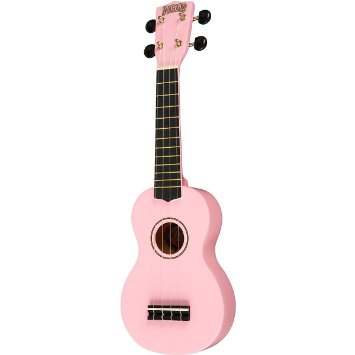
\includegraphics[width=5cm]{../img/ukulele.jpg}
\end{Slide}


\fi